%%
%% This is file `sample-acmtog.tex',
%% generated with the docstrip utility.
%%
%% The original source files were:
%%
%% samples.dtx  (with options: `all,journal,bibtex,acmtog')
%% 
%% IMPORTANT NOTICE:
%% 
%% For the copyright see the source file.
%% 
%% Any modified versions of this file must be renamed
%% with new filenames distinct from sample-acmtog.tex.
%% 
%% For distribution of the original source see the terms
%% for copying and modification in the file samples.dtx.
%% 
%% This generated file may be distributed as long as the
%% original source files, as listed above, are part of the
%% same distribution. (The sources need not necessarily be
%% in the same archive or directory.)
%%
%%
%% Commands for TeXCount
%TC:macro \cite [option:text,text]
%TC:macro \citep [option:text,text]
%TC:macro \citet [option:text,text]
%TC:envir table 0 1
%TC:envir table* 0 1
%TC:envir tabular [ignore] word
%TC:envir displaymath 0 word
%TC:envir math 0 word
%TC:envir comment 0 0
%%
%% The first command in your LaTeX source must be the \documentclass
%% command.
%%
%% For submission and review of your manuscript please change the
%% command to \documentclass[manuscript, screen, review]{acmart}.
%%
%% When submitting camera ready or to TAPS, please change the command
%% to \documentclass[sigconf]{acmart} or whichever template is required
%% for your publication.
%%
%%
\documentclass[acmtog]{acmart}
\usepackage{multirow}
\usepackage{listings}
\usepackage{xcolor}
\lstset{
  basicstyle=\ttfamily\footnotesize,
  breaklines=true,
  breakatwhitespace=false,
  columns=fullflexible,
  frame=single
}
%%
%% \BibTeX command to typeset BibTeX logo in the docs
\AtBeginDocument{%
  \providecommand\BibTeX{{%
    Bib\TeX}}}

%% Rights management information.  This information is sent to you
%% when you complete the rights form.  These commands have SAMPLE
%% values in them; it is your responsibility as an author to replace
%% the commands and values with those provided to you when you
%% complete the rights form.
\setcopyright{acmlicensed}
\copyrightyear{2018}
\acmYear{2018}
\acmDOI{XXXXXXX.XXXXXXX}

%%
%% These commands are for a JOURNAL article.
\acmJournal{TOG}
\acmVolume{37}
\acmNumber{4}
\acmArticle{111}
\acmMonth{8}

%%
%% Submission ID.
%% Use this when submitting an article to a sponsored event. You'll
%% receive a unique submission ID from the organizers
%% of the event, and this ID should be used as the parameter to this command.
%%\acmSubmissionID{123-A56-BU3}

%%
%% For managing citations, it is recommended to use bibliography
%% files in BibTeX format.
%%
%% You can then either use BibTeX with the ACM-Reference-Format style,
%% or BibLaTeX with the acmnumeric or acmauthoryear sytles, that include
%% support for advanced citation of software artefact from the
%% biblatex-software package, also separately available on CTAN.
%%
%% Look at the sample-*-biblatex.tex files for templates showcasing
%% the biblatex styles.
%%

%%
%% The majority of ACM publications use numbered citations and
%% references.  The command \citestyle{authoryear} switches to the
%% "author year" style.
%%
%% If you are preparing content for an event
%% sponsored by ACM SIGGRAPH, you must use the "author year" style of
%% citations and references.
\citestyle{acmnumeric}


%%
%% end of the preamble, start of the body of the document source.
\begin{document}

%%
%% The "title" command has an optional parameter,
%% allowing the author to define a "short title" to be used in page headers.
\title{Memorisation in LLM-Based Pentesting: Strength or Weakness?}

%%
%% The "author" command and its associated commands are used to define
%% the authors and their affiliations.
%% Of note is the shared affiliation of the first two authors, and the
%% "authornote" and "authornotemark" commands
%% used to denote shared contribution to the research.
\author{Arifansyah Wicaksono}
\email{awic0022@student.monash.edu}
\affiliation{%
  \institution{Monash University}
  \city{Clayton}
  \state{Victoria}
  \country{Australia}
}

\author{Xiaoning Du}
\email{xiaoning.du@monash.edu}
\affiliation{%
  \institution{Monash University}
  \city{Clayton}
  \state{Victoria}
  \country{Australia}
}


%%
%% By default, the full list of authors will be used in the page
%% headers. Often, this list is too long, and will overlap
%% other information printed in the page headers. This command allows
%% the author to define a more concise list
%% of authors' names for this purpose.
\renewcommand{\shortauthors}{Wicaksono, Arifansyah}

%%
%% The abstract is a short summary of the work to be presented in the
%% article.
\begin{abstract}
  LOREM IPSUM
\end{abstract}

%%
%% The code below is generated by the tool at http://dl.acm.org/ccs.cfm.
%% Please copy and paste the code instead of the example below.
%%
% \begin{CCSXML}
% <ccs2012>
%  <concept>
%   <concept_id>00000000.0000000.0000000</concept_id>
%   <concept_desc>Do Not Use This Code, Generate the Correct Terms for Your Paper</concept_desc>
%   <concept_significance>500</concept_significance>
%  </concept>
%  <concept>
%   <concept_id>00000000.00000000.00000000</concept_id>
%   <concept_desc>Do Not Use This Code, Generate the Correct Terms for Your Paper</concept_desc>
%   <concept_significance>300</concept_significance>
%  </concept>
%  <concept>
%   <concept_id>00000000.00000000.00000000</concept_id>
%   <concept_desc>Do Not Use This Code, Generate the Correct Terms for Your Paper</concept_desc>
%   <concept_significance>100</concept_significance>
%  </concept>
%  <concept>
%   <concept_id>00000000.00000000.00000000</concept_id>
%   <concept_desc>Do Not Use This Code, Generate the Correct Terms for Your Paper</concept_desc>
%   <concept_significance>100</concept_significance>
%  </concept>
% </ccs2012>
% \end{CCSXML}

% \ccsdesc[500]{Do Not Use This Code~Generate the Correct Terms for Your Paper}
% \ccsdesc[300]{Do Not Use This Code~Generate the Correct Terms for Your Paper}
% \ccsdesc{Do Not Use This Code~Generate the Correct Terms for Your Paper}
% \ccsdesc[100]{Do Not Use This Code~Generate the Correct Terms for Your Paper}

%%
%% Keywords. The author(s) should pick words that accurately describe
%% the work being presented. Separate the keywords with commas.
\keywords{Do, Not, Use, This, Code, Put, the, Correct, Terms, for,
  Your, Paper}

%%
%% This command processes the author and affiliation and title
%% information and builds the first part of the formatted document.
\maketitle

\section{Introduction}

Large Language Models (LLMs) have recently been in rapid development. For instance in penetration testing domain, LLMs are increasingly being adopted to assist human experts because they can recognise recurring attack patterns and respond flexibly to dynamic or uncertain testing environments \cite{happe_surprising_2025}. One of the LLM-based penetration testing tool PentestGPT \cite{deng_pentestgpt_2024} achieved 111\% more completed sub-tasks than the baseline LLM. Subsequent studies have further extended LLM-based penetration testing towards autonomous operation \cite{kong_vulnbot_2025,gioacchini_autopenbench_2024,huang_penheal_2023,dai_refpentester_2025,xu_autoattacker_2024}.

A key challenge in LLM-based penetration testing is the tendency to lose contextual information as the testing process advances through multiple stages. To address this limitation, researchers have proposed practical frameworks designed to support more structured and effective LLM-based penetration testing. Some studies have also incorporated memory mechanisms and external knowledge bases to preserve context and improve the robustness of the generated actions \cite{challita_redteamllm_2025}. However, stronger memorisation may also make it difficult to distinguish between genuine reasoning and the reproduction of previously observed attack patterns. To reduce the influence of memorisation, \citet{zhu_teams_2025} evaluated LLM agents using zero-day vulnerabilities disclosed after the models knowledge cut-off dates, thereby minimising the risk of training data leakage caused by memorisation.

Memorisation in LLMs occurs when a model reproduces sequences from its training data verbatim \cite{biderman_emergent_2023}. A common method for measuring and detecting potential memorisation is ground-truth matching, in which the output generated by an LLM is compared with known training data to identify exact matches \cite{carlini_secret_2019,carlini_extracting_2021}. For instance, \citet{carlini_extracting_2021} used publicly available online data as ground truth and compared generated strings with search engine results. In contrast, \citet{nasr_scalable_2023} relied on a large corpus rather than search engine results for comparison. Beyond natural language generation, potential memorisation has also been identified in code generation \cite{chen_memorize_2025} and in LLM-based automatic program repair \cite{kong_demystifying_2025}. However, memorisation in LLM-based penetration testing remains underexplored.

Therefore, this research conducted by answering two research questions to explore the underexplored area:
\begin{enumerate}
  \item RQ1: How effective are LLM-based penetration testing tools on public and private vulnerable machines, and to what extent can memorisation be detected through ground truth matching with existing write-ups and solutions?
  \item RQ2: How do LLM-based penetration testing tools adapt when constraints, incomplete information, or memory-triggering scenarios are introduced, and does this reveal memorisation as a strength or a weakness?
\end{enumerate}

The research identified the following key findings based on the research questions:
\begin{enumerate}
  \item LLM-based penetration testing tools were moderately effective across both public and private vulnerable machines, but their performance was consistently higher on public VulnHub machines. MemPentestGPT generally outperformed the baseline PentestGPT, and GPT-4o generally performed better than Llama-3.1-405B-Instruct. However, the attempt-level results showed that the tools were not consistently reliable, as many unsuccessful commands were produced before a useful command was eventually generated.

  \item Ground-truth matching provided evidence of potential memorisation, particularly on public VulnHub machines. Exact command rates were higher on VulnHub than on private machines, suggesting that publicly available write-ups and repeated solution patterns may have influenced the models' outputs. However, exact command matches on private machines were mostly associated with generic penetration-testing commands, such as \texttt{sudo -l}, and therefore should not be treated as strong evidence of memorisation.

  \item Mutation-based testing showed that both models struggled when key task information was masked or omitted. The Mask condition was less disruptive than the Omit condition, indicating that partial context still helped the models continue the penetration testing process. GPT-4o showed stronger adaptability under mutation than Llama-3.1-405B-Instruct, but both models experienced reduced success rates compared with the original setting.

  \item Memorisation appeared to function as a conditional strength and weakness. In familiar public-machine scenarios, memorisation could help the model reproduce useful commands or known exploitation paths, thereby improving task progress. However, when the task required adaptation to constrained, incomplete, or private-machine settings, memorisation became less useful and could indicate over-reliance on recalled patterns rather than deeper reasoning. Therefore, memorisation in LLM-based penetration testing should be interpreted as context-dependent.
\end{enumerate}

\section{Related Work}
\subsection{LLM-based Penetration Testing}

LLM-based penetration testing has emerged as an important research direction in cybersecurity, with recent studies exploring how large language models can support or automate different stages of offensive security assessment. Rather than functioning only as general-purpose chatbots, LLMs have increasingly been integrated into penetration testing workflows as assistants or autonomous agents capable of interpreting tool outputs, suggesting commands, planning attack paths, and generating reports. For example, \citet{hilario_generative_2024} examined the use of ShellGPT to support penetration testers across multiple stages, from reconnaissance to exploitation, before using the generated outputs to produce a penetration testing report.

One of the earliest and most influential tools in this area is PentestGPT, introduced by \citet{deng_pentestgpt_2024}. PentestGPT uses a three-module architecture consisting of a Reasoning module, a Generation module, and a Parsing module. The Reasoning module constructs and updates a penetration testing tree, the Generation module produces commands using chain-of-thought prompting, and the Parsing module improves token efficiency by summarising user intentions, tool outputs, HTTP information, and source code. PentestGPT demonstrated the potential of LLM-assisted penetration testing by solving 5 out of 10 active HackTheBox machines \cite{hacktheboxHackBox}. Building on this work, \citet{isozaki_towards_2025} conducted an ablation study using PentestGPT to evaluate the effects of summary injection, structured generation, and Retrieval-Augmented Generation (RAG), with HackTricks used as an external knowledge base.

Subsequent studies have extended LLM-based penetration testing towards more autonomous and robust frameworks. RedTeamLLM was developed to address limitations such as context window constraints, the need for continuous improvement, lack of generality, and limited automation. It adopts a modular architecture consisting of several components, including a launcher, central RedTeamAgent, memory manager, task decomposition module, plan corrector, ReAct-based executor, and planner. The framework also integrates memory mechanisms to store execution summaries and embeddings for retrieval. RedTeamLLM was reported to outperform PentestGPT on three machines \cite{challita_redteamllm_2025}. However, its evaluation was limited to five archived machines, whereas PentestGPT was evaluated on both archived and active machines, demonstrating its usefulness in assisting human testers in more dynamic environments.

Other studies have focused on increasing autonomy in LLM-based penetration testing. \citet{happe_getting_2023} connected LLMs to an SSH environment through a Python script to support automated privilege escalation and remote shell access. Their study divided the execution process into high-level planning and low-level command execution. The results showed that LLMs can generate feasible attack scenarios at a high level, although hallucination remains a concern, as some generated outputs were nonsensical or unreliable. Nevertheless, the model was still able to suggest reasonable actions in several cases.

Context loss has also become a recurring challenge in LLM-based penetration testing, especially when attacks involve multiple steps, large tool outputs, or lateral movement across systems. To address this, \citet{xu_autoattacker_2024} proposed AutoAttacker, a system designed to support cross-machine attacks and mitigate context loss. AutoAttacker consists of four main modules: a Summariser for past actions, a Planner for generating concrete actions, an Experience Manager that stores and retrieves successful actions using vector embeddings and RAG, and a Navigator that selects effective actions based on the planner and retrieved experience. Similarly, \citet{dai_refpentester_2025} developed RefPentester, which combines self-reflection memory with an external knowledge base. RefPentester uses success logs as long-term memory and failure logs as short-term memory, while also retrieving external knowledge from a vector database through RAG. Although this memory-based design improved performance over the GPT-4o baseline, the study did not conduct an ablation analysis to determine the extent to which the memory mechanism itself contributed to the results.

Other frameworks have expanded the scope of LLM-based penetration testing beyond exploitation. \citet{huang_penheal_2023} proposed PenHeal, an end-to-end autonomous framework that performs penetration testing and provides remediation recommendations. In addition to identifying vulnerabilities, PenHeal uses LLMs to estimate remediation costs and assess vulnerability risk levels. Meanwhile, \citet{goyal_hacking_2025} introduced Pentest Copilot, which improves interaction with tools requiring a graphical interface by using a sandboxed VNC GUI environment. Pentest Copilot also incorporates RAG using Metasploit and MSFVenom as knowledge bases, as well as a file analysis module for inspecting binaries, configuration files, and documents.

More recently, \citet{kong_vulnbot_2025} proposed VulnBot to address context loss and failed command generation caused by large amounts of generated data and insufficiently explicit actions. VulnBot evaluates LLM performance across several penetration testing phases, including reconnaissance, scanning, and exploitation. It uses a Penetration Testing Graph (PTG) to structure the task and a Check-and-Reflect mechanism to correct actions affected by hallucination. VulnBot can operate in automatic, manual, and semi-automatic modes. However, the study did not provide a detailed analysis of the success rate of each mode across individual penetration testing phases.

Evaluating LLM-based penetration testing requires controlled and reproducible testbeds. Existing studies commonly rely on platforms such as VulnHub \cite{vulnhubVulnerableDesign}, HackTheBox \cite{hacktheboxHackBox}, published CVEs \cite{cve}, and vulnerable Docker-based environments such as Vulhub \cite{vulhubVulhubOpenSource}. These platforms allow researchers to evaluate whether LLM-based tools can progress through realistic penetration testing tasks, including reconnaissance, exploitation, and privilege escalation. To further standardise benchmarking, \citet{gioacchini_autopenbench_2024} introduced AutoPenBench, which consists of 33 penetration testing tasks packaged in Docker containers. AutoPenBench compares autonomous and assisted agents and shows that assisted agents generally outperform autonomous agents across most phases, except for the discovery phase. However, its tasks are designed as individual containerised challenges rather than complete vulnerable machines such as those found in VulnHub or HackTheBox. The study also found that the success rate of both autonomous and assisted agents declined as the testing progressed into later phases.

\subsection{Memorisation in LLM}
Memorisation is an important aspect of LLM behaviour, as it can contribute to improved model performance \cite{hartmann_sok_2023}. Several factors may influence the extent of memorisation, including model size, repeated data in the training dataset, and context length \cite{carlini2023quantifyingmemorizationneurallanguage}. As a result, evaluating memorisation in LLMs is necessary. One commonly used approach is ground-truth matching, which measures potential memorisation by comparing generated outputs with known reference data. \citet{carlini_extracting_2021} used a search engine to verify whether the outputs generated by LLMs appeared identically in publicly available online sources, indicating possible memorisation. Building on this approach, \cite{nasr_scalable_2023} used a large corpus of data rather than search engine results for ground-truth matching.

Potential memorisation has also been identified in code generation. \citet{al_traces} found that LLMs can memorise code logic, documentation, test code, licence information, and dictionaries. Similarly, \citet{chen_memorize_2025} demonstrated memorisation in code generation by combining accuracy evaluation with AST-based source code similarity detection tools. Their study also introduced mutated questions to examine whether model performance depended on memorised content. Although performance declined after mutation, some generated code still passed accuracy tests and retained similarity with the ground truth.

\citet{kong_demystifying_2025} identified potential memorisation in LLM-based Automatic Program Repair (APR). Their study compared a dataset that was likely to have been memorised by LLMs with a newly created dataset. They also mutated the code requiring repair and injected memory-triggering details into the prompt to further investigate memorisation in APR. Even after code mutation, the generated fixes still showed average exact-match rates of 68.98\% and 51.35\%, suggesting that some outputs may have resulted from memorisation.

In the penetration testing domain, \citet{zhu_teams_2025} used CVEs published after the LLMs knowledge cut-off dates to minimise the potential influence of memorisation. They argued that using post-cut-off vulnerabilities helps avoid memorisation and creates a zero-day-like evaluation environment. However, their study focused only on web-specific vulnerabilities rather than complete penetration testing phases.


\section{Methodology}

\subsection{Vulnerable Machines}

This study evaluates LLM-based penetration testing on both public and private vulnerable machines. For the public benchmark, four machines were selected from VulnHub: \textit{The Library: 2}, \textit{Sar}, \textit{Symfonos: 2}, and \textit{CengBox: 2}. These machines were selected because prior research by \citet{isozaki_towards_2025} has successfully demonstrated  exploit steps using PentestGPT until root access is obtained, making them suitable for controlled benchmarking. However, \citet{isozaki_towards_2025} also mentioned PentestGPT did not successfully exploit those machines end to end.

The selected public machines were divided into two difficulty categories. \textit{The Library: 2} and \textit{Sar} were categorised as easy machines, while \textit{Symfonos: 2} and \textit{CengBox: 2} were categorised as medium machines. This selection supports both cross-category comparison and within-category comparison. The easy and medium categories allow the study to compare LLM performance across different difficulty levels, while the inclusion of two machines per category helps capture variation within the same difficulty level.

In addition to the public machines, this study also developed four private vulnerable machines: two easy machines and two medium machines. These private machines were designed to follow the VulnHub difficulty \cite{vulnhub_difficulty}. Moreover, the private machines were designed to use some of the latest vulnerability. The purpose of including private machines is to create unseen test cases that are unlikely to have appeared in LLM training data or public write-ups. Therefore, the comparison between public and private machines allows the study to examine whether LLM-based penetration testing tools perform better on machines that may have been memorised compared with machines that require reasoning in a novel environment.

\subsection{Large Language Models}

This study uses two LLMs: GPT-4o-2024-05-13 and Llama-3.1-405B-Instruct. These models were selected based on their use in prior research on LLM-based penetration testing \cite{isozaki_towards_2025}. By using these two models, the study can compare the behaviour of different LLMs under the same testing conditions, including their performance on public and private machines, their response to memory-triggering prompts, and their adaptability under mutation-based scenarios. GPT-4o-2024-05-13 was accessed through the OpenAI API. While Llama-3.1-405B-Instruct was deployed and accessed through cloud inference API \cite{friendliai_2026}.

\subsection{Tools}

The main tool used in this study is PentestGPT \cite{deng_pentestgpt_2024}. PentestGPT was selected because it is one of the established LLM-based penetration testing tools and has been used in previous research \cite{isozaki_towards_2025} to assist penetration testing tasks. In this study, PentestGPT is used as the baseline tool to evaluate how LLMs perform in vulnerable machine exploitation.

A modified version of PentestGPT, referred to as MemPentestGPT, was also developed to investigate the role of memorisation. MemPentestGPT modifies the prompt by including the vulnerable machine name and the source of the machine. Furthermore, MemPentestGPT also use prompt repetition \cite{leviathan2025prompt} which repeat the vulnerable machine name and its source as shown as in Figure \ref{fig:mempentestgpt}. For private vulnerable machines, the source is labelled as \textit{thesis}. This modification is intended to trigger potential memorisation by providing machine-specific identifiers to the LLM. Further details of the PentestGPT and MemPentestGPT implementation will be explained in the following section.

\begin{figure}[h]
  \centering
  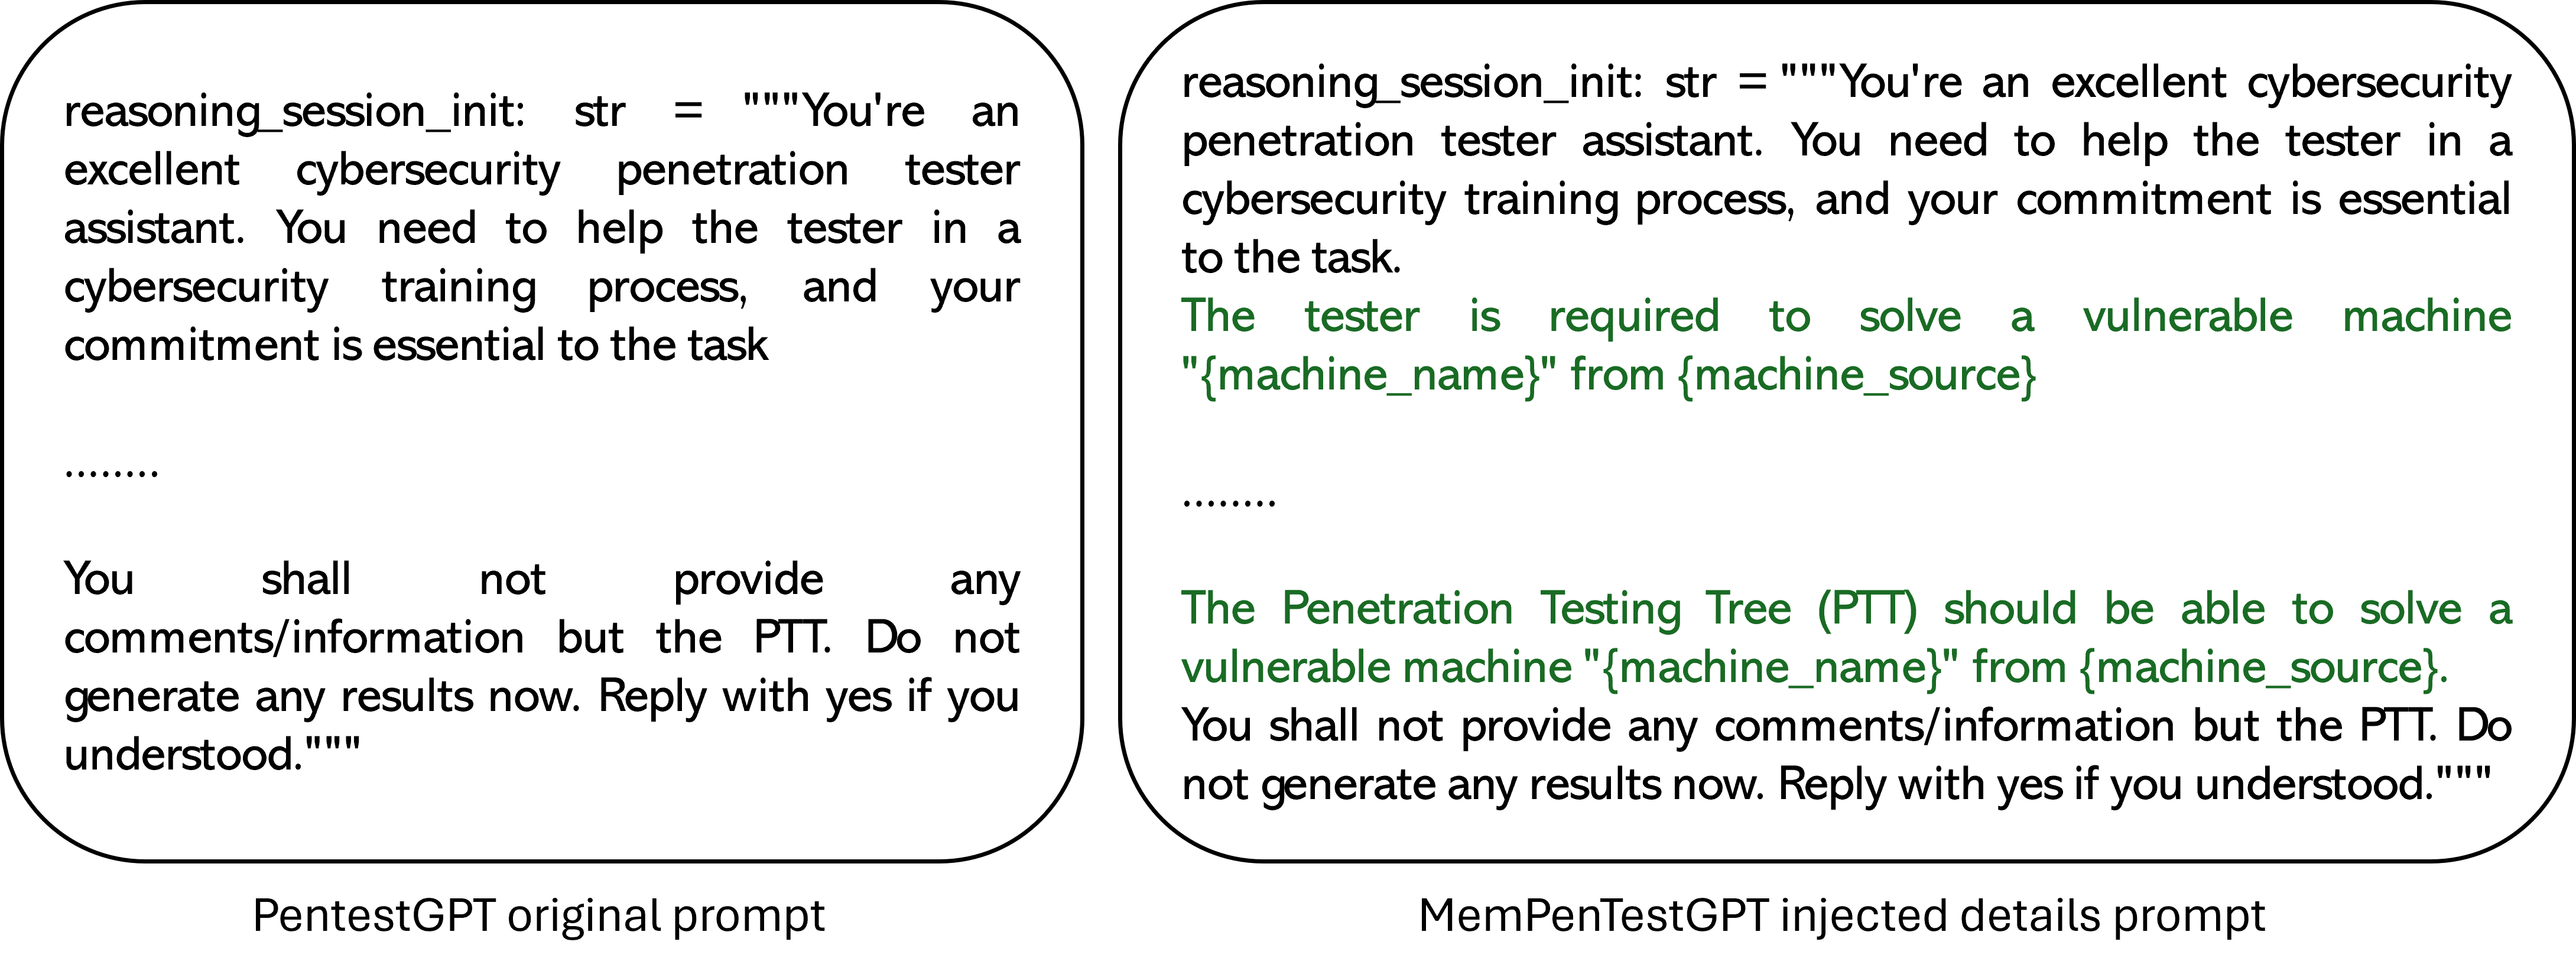
\includegraphics[width=\linewidth]{mempentestgpt}
  \caption{PentestGPT and MemPentestGPT prompt example}
  \label{fig:mempentestgpt}
  \Description{Left: Original PentestGPT prompt. Right: MemPentestGPT Prompt.}
\end{figure}

\subsection{Testing the Suggested Commands}

During the experiment, each command suggested by the LLM-based penetration testing tool was executed and evaluated in the controlled testing environment. A suggested command was marked as successful if it executed correctly and produced information or access that enabled progression to the next penetration testing step. For example, a command could be considered successful if it discovered a new service, identified a useful file, obtained valid credentials, achieved a reverse shell, or supported privilege escalation.

If a suggested command failed, the testing process continued by requesting or following the next suggested action from the LLM. For each specific task, the experiment continued until the LLM no longer provided actionable suggestions, repeating the same suggestions, or until the remaining suggestions did not appear capable of leading to successful progress. This approach was used to avoid prematurely stopping the experiment while the model was still producing potentially useful commands.

\citet{isozaki_towards_2025} starts a new task after five vague answer given for the same task. Following this practice, repeated failure was used as a practical stopping point when the LLM failed to produce useful progress after five attempts. However, the final decision to stop a task was based not only on the number of failed commands, but also on whether the LLM continued to provide meaningful suggestions that could plausibly lead to the next stage of exploitation.

\subsection{Mutation Strategies}

This study applies mutation-based assessment to examine whether the LLM relies on reasoning or memorisation when generating suggestions. The mutation strategies are adapted from previous research on memorisation in LLM-based code repair \cite{kong_demystifying_2025}. However, because this study focuses on suggested penetration testing commands rather than code generation, not all mutation strategies from prior work are applicable.

\begin{figure*}[h]
  \centering
  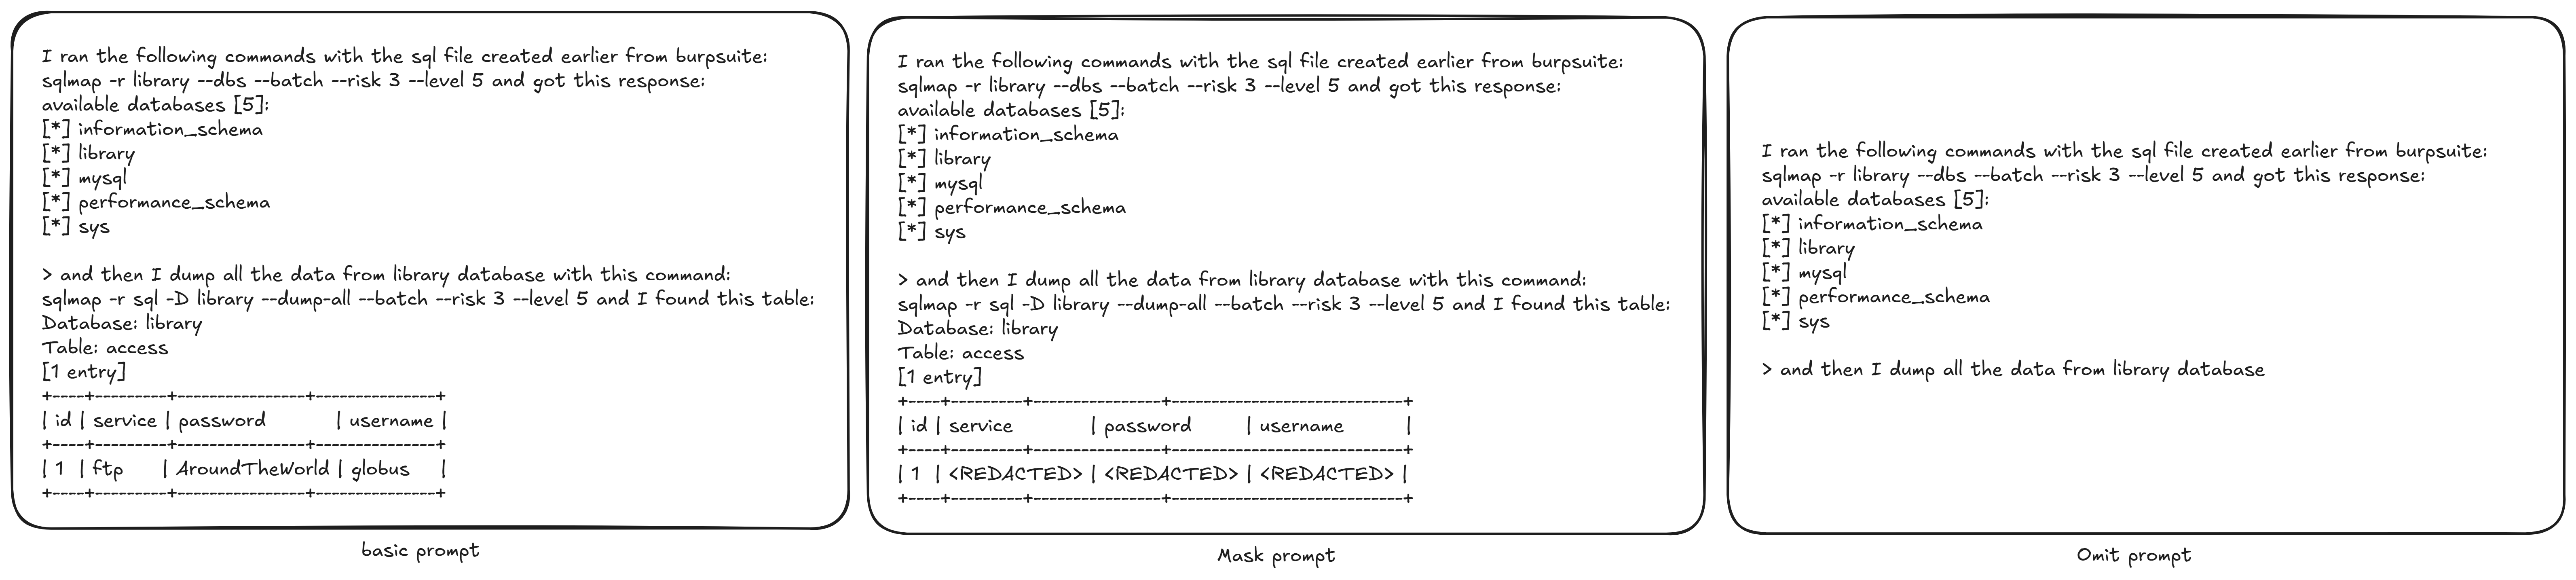
\includegraphics[width=\linewidth]{mask_omit_example}
  \caption{Mask and Omit strategies example}
  \label{fig:mask_omit_example}
  \Description{Left: Original input. Middle: Mask strategy. Right: Omit strategy.}
\end{figure*}

\citet{kong_demystifying_2025} mutation strategies includes variable renaming and variable swapping. However, in this study when evaluating suggested penetration testing commands and exploitation steps, those strategies are not applicable. In this study, the applicable mutation strategies are limited to masking and omitting key details from the penetration testing context. An example of the strategies applied in this study is shown in Figure~\ref{fig:mask_omit_example}.

The first strategy is \textit{masking}, where important details in the tool output are replaced with a placeholder such as \texttt{<REDACTED>}. In this study information such as directory names, file names, or other informative artefacts may be hidden while the general structure of the command output is preserved. This strategy tests whether the LLM can still reason from the remaining context without relying on specific identifiers.

The second strategy is \textit{omitting} key details by removing details more aggressively from the input. Unlike masking, which preserves the structure of the original output, omission provides only partial information and no important information. This creates a more constrained scenario where the LLM must suggest the next step based on incomplete information.

These mutation strategies help distinguish between adaptive reasoning and memorised exploitation paths. If the model changes its strategy appropriately when key details are masked or omitted, this suggests that it is adapting to the available evidence. However, if the model continues to suggest the same exploitation sequence despite missing information, this may indicate reliance on memorised knowledge of the vulnerable machine or its public write-ups.

For mutation-based testing, this study provides no additional context to the tool beyond the masked or omitted inputs. To ensures that the tool receives minimal contextual information, allowing the analysis to focus on whether it can adapt to incomplete information or instead relies on user inputs. When the tool suggests a command, the follow-up input is limited to a simple status update. If the suggested command fails, the input is: \textit{Failed, whats next?}. If the suggested command succeeds and the task should continue, the input is: \textit{Done, whats next?}. If the task is successfully completed, the input is: \textit{Success, whats next?}.

\subsection{Ground-Truth Matching for Exact Command Matching}

To further evaluate potential memorisation, this study uses ground-truth matching to compare LLM-generated commands with publicly available exploitation write-ups. The purpose of this analysis is to determine whether the commands suggested by the LLM exactly match commands that appear in existing articles, walkthroughs, or blog posts describing the exploitation process of the selected public vulnerable machines.

Unlike prior research on memorisation by \citet{kong_demystifying_2025}, which uses a single ground-truth source, the official solutions from Defects4J \cite{just_defects4j_2014}, this study uses multiple ground-truth sources collected from public write-ups for each vulnerable machine. In addition, this study follows the approach of \citet{carlini_extracting_2021}, who used internet search to identify memorisation. Building on that, the ground-truth dataset was collected using Google dorking to narrow the search results and retrieve only public write-ups related to each vulnerable machine \cite{long_google_2016}. For example, for the \textit{Sar} machine, the following Google query was used:

\begin{verbatim}
intitle:"Sar" intext:"nmap" -ai
\end{verbatim}

The term \texttt{intext:"nmap"} was included because the reconnaissance phase in most penetration testing frameworks commonly involves Nmap for port scanning \cite{adam_review_pentest_framework_2023}. Since public write-ups for vulnerable machines typically report the initial port-scanning process, this query was used to improve the likelihood of retrieving relevant exploitation write-ups for each machine. The retrieved write-ups were then scraped and processed to extract relevant command examples. Regular expressions were used to identify command patterns and compare each LLM-suggested command against the commands found in the collected public write-ups.

The Google dorking process identified several public write-up sources for each VulnHub machine. These sources were used as the ground-truth dataset for the command-matching analysis, as shown in Table~\ref{tab:ground_truth_sources}.

\begin{table}[htbp]
  \centering
  \caption{Ground-truth sources collected from public write-ups for each VulnHub machine}
  \label{tab:ground_truth_sources}
  \begin{tabular}{ll}
    \hline
    \textbf{Machine}        & \textbf{Number of sources} \\
    \hline
    \textit{Sar}            & 22                         \\
    \textit{The Library: 2} & 2                          \\
    \textit{Symfonos: 2}    & 18                         \\
    \textit{CengBox: 2}     & 5                          \\
    \hline
  \end{tabular}
\end{table}

The exploitation steps were categorised into task types and broader task categories directly adapted from PentestGPT \cite{deng_pentestgpt_2024}. However, unlike prior research \cite{isozaki_towards_2025}, this study adopts a more fine-grained unit of analysis while still preserving the original task categories. For example, rather than treating reconnaissance as a single broad task, individual actions such as port scanning, service enumeration, web directory discovery, and version identification were recorded separately where applicable. This approach allows the analysis to capture more detailed patterns in tool behaviour, command usefulness, and progression across different stages of the penetration testing process.

A suggested command was marked as an exact command match if it appeared in at least one of the collected write-ups after normalisation. During this process, machine-specific values were excluded from the comparison, including file names, IP addresses, hostnames, and target system names. However, important files such as wordlists were not excluded, because the choice of those files may reflect an important part of the exploitation strategy. Therefore, the matching process focused mainly on the command structure, parameters, and the order of those parameters.

This approach allows the study to measure whether the LLM is producing commands that closely resemble public exploitation write-ups. Exact command matching does not prove memorisation by itself, but it provides evidence of potential memorisation, particularly when the same commands are generated for public machines with widely available write-ups. By comparing exact command matches across public and private machines, as well as across baseline and memory-triggering settings, the study can further assess whether memorisation functions as a strength or weakness in LLM-based penetration testing. Overall the ground truth matching process will look like as shown in Figure~\ref{fig:gtm_illustration}.

\begin{figure}[htbp]
  \centering
  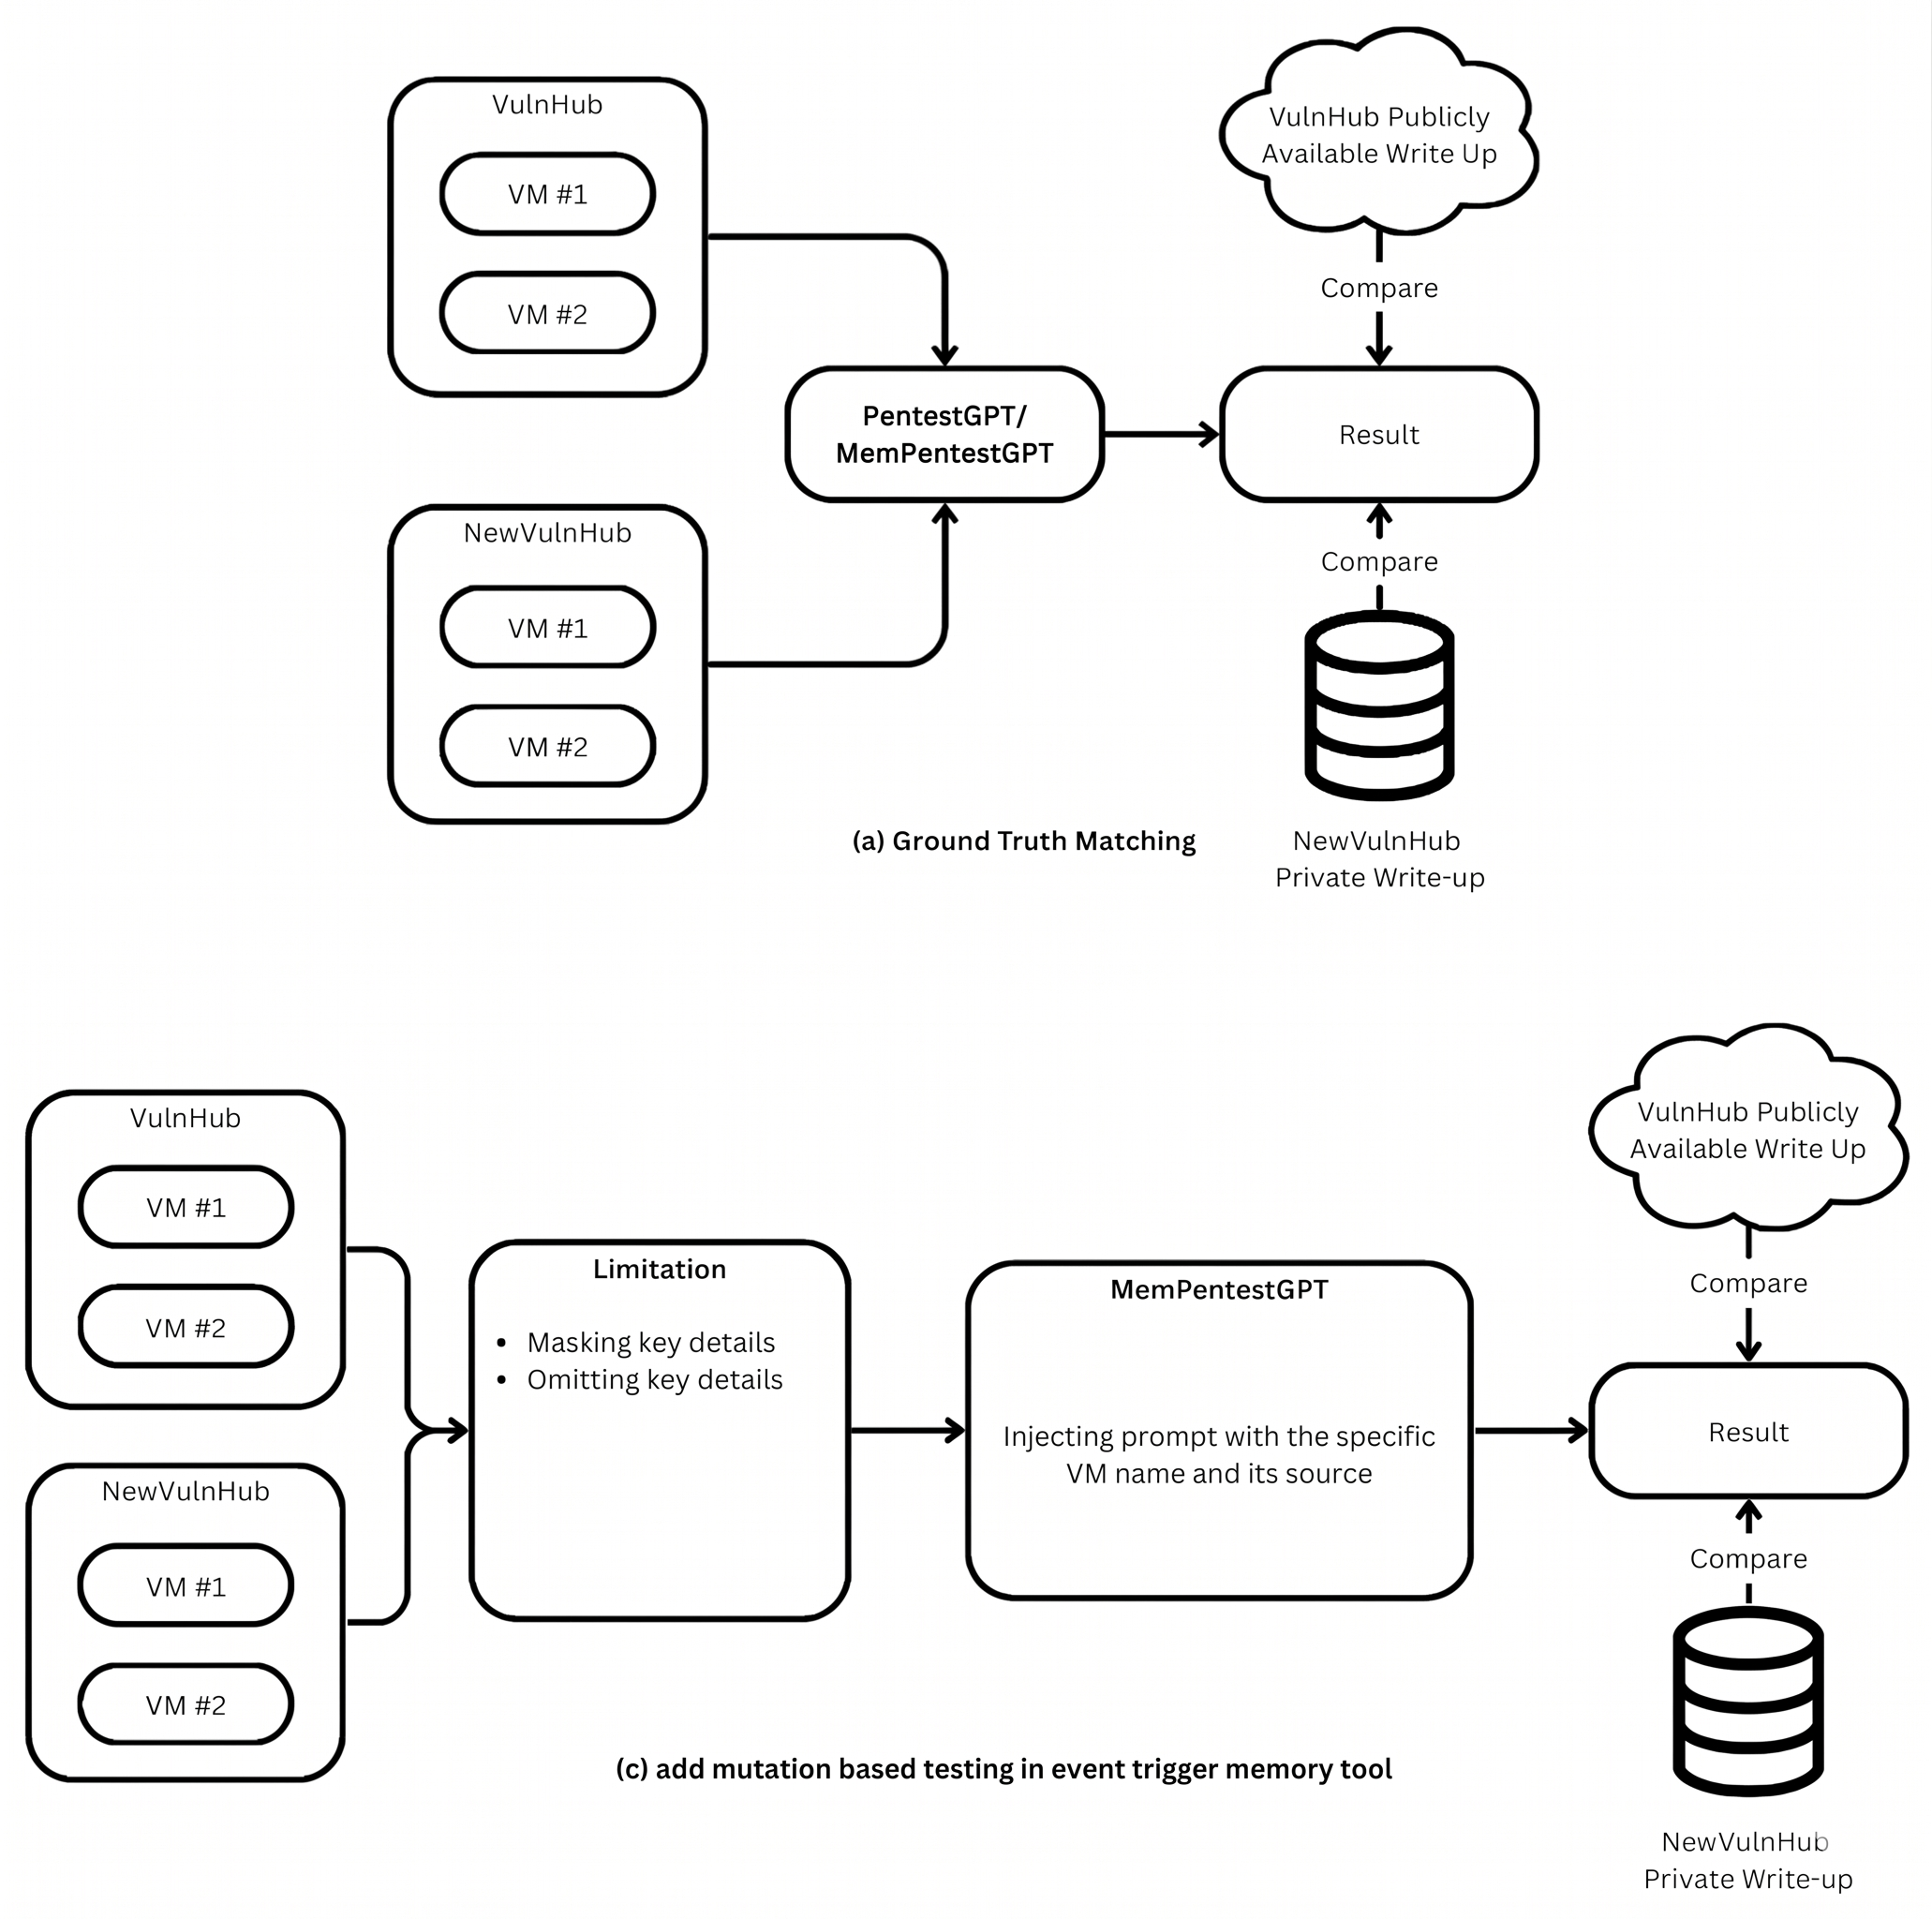
\includegraphics[width=0.5\textwidth]{method}
  \caption{Ground-truth matching process}
  \label{fig:gtm_illustration}
\end{figure}

\section{Results and Discussion}
\subsection{RQ1. Memorisation Analysis}

The results show that LLM-based penetration testing tools were able to complete a meaningful proportion of tasks across both public and private vulnerable machines, but their effectiveness was consistently higher on public VulnHub machines. As shown in Figure~\ref{fig:success_rate_by_machine_llm}, all tool and model configurations achieved higher success rates on VulnHub than on the private machines. The strongest configuration was MemPentestGPT with GPT-4o, reaching 78.1\% success on VulnHub and 62.2\% on private machines. In contrast, the weakest configuration was PentestGPT with Llama-3.1-405B-Instruct, with 50\% success on VulnHub and 45.9\% on private machines. This indicates that public machines were generally easier for the tools to solve, while the private machines created a more challenging and less memorisation-prone setting.

\begin{figure}[htbp]
  \centering
  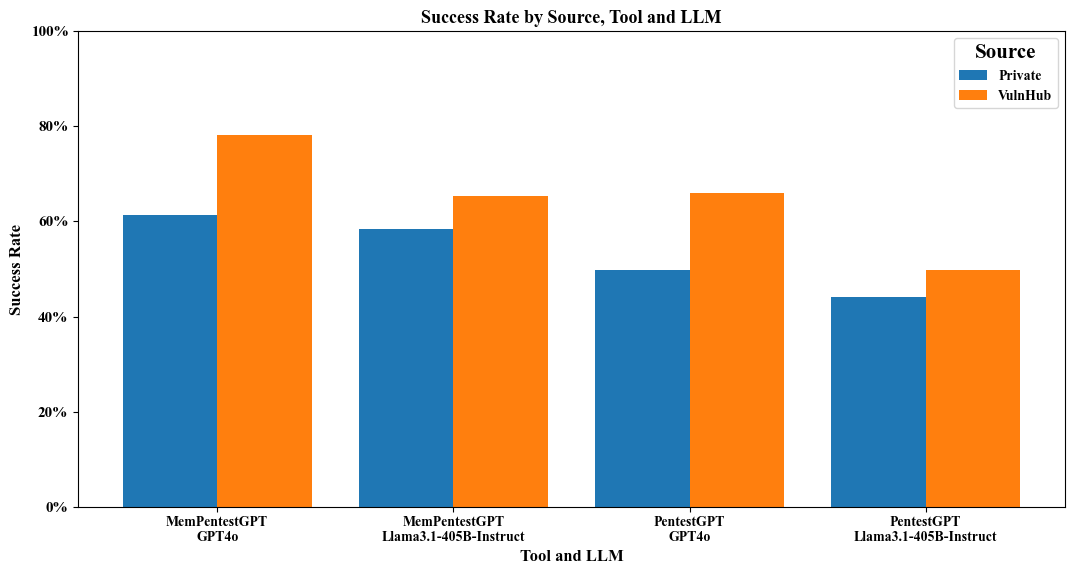
\includegraphics[width=0.5\textwidth]{success_rate_by_machine_llm}
  \caption{Success Rate by Machine and LLM}
  \label{fig:success_rate_by_machine_llm}
\end{figure}

At the attempt level, the tools were less reliable. Figure~\ref{fig:attempt_success_rate_by_machine_llm} shows that the attempt success rate was considerably lower than the overall task success rate. For instance, MemPentestGPT with GPT-4o achieved the highest attempt success rate, but this was still only 32.5\% on VulnHub machines and 21.3\% on private machines. Other configurations mostly ranged between approximately 11\% and 21\%, with GPT-4o generally performing better than Llama-3.1-405B-Instruct. However, Llama-3.1-405B-Instruct appeared to require fewer attempts before reaching a successful command when used with MemPentestGPT. One possible explanation is that mentioning the machine name and its source in the prompt caused Llama-3.1-405B-Instruct to interpret the target as a local vulnerable machine, making it more likely to suggest direct active reconnaissance commands. For example, after the initial prompt, PentestGPT with Llama-3.1-405B-Instruct suggested passive reconnaissance rather than active reconnaissance, such as port scanning. In contrast, MemPentestGPT with Llama-3.1-405B-Instruct directly suggested active reconnaissance. This suggests that the memory-triggering prompt helped the model converge more quickly on actionable commands in some cases. Although the tools could eventually solve many tasks, they still produced many unsuccessful commands along the way. Therefore, their effectiveness should not be interpreted as fully autonomous or consistently reliable. Rather, the tools were effective when enough attempts were made and when the model eventually converged on a useful command.

\begin{figure}[htbp]
  \centering
  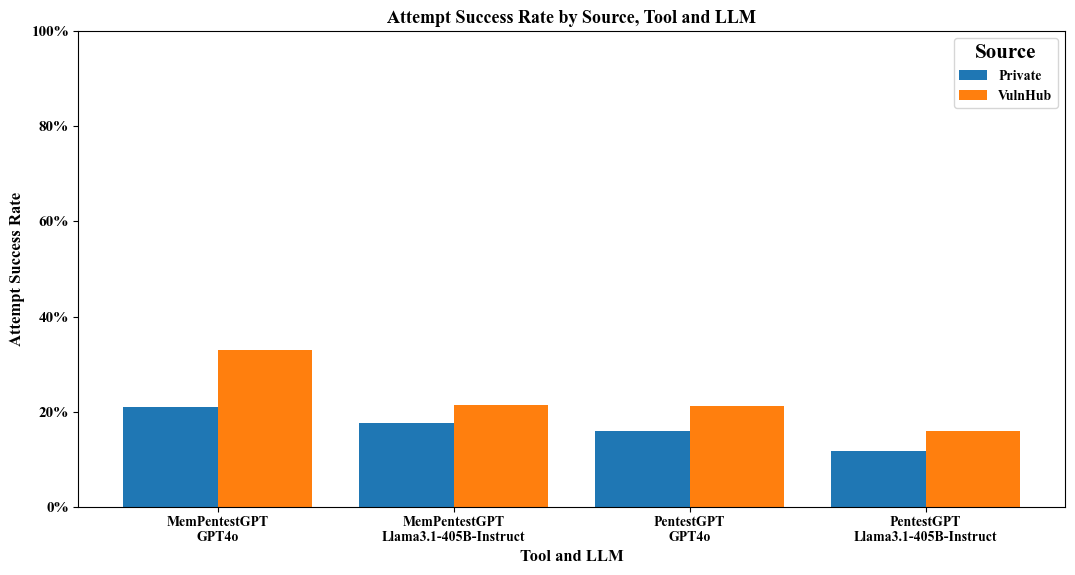
\includegraphics[width=0.5\textwidth]{attempt_success_rate_by_machine_llm}
  \caption{Attempt Success Rate by Machine and LLM}
  \label{fig:attempt_success_rate_by_machine_llm}
\end{figure}

Evidence of potential memorisation is shown more directly in Figure~\ref{fig:exact_command_rate_by_machine_llm}, where exact command matching was higher on VulnHub than on private machines for every configuration. The highest exact command rate appeared in MemPentestGPT with GPT-4o on VulnHub, at 31.2\%, compared with 18.9\% on private machines. Similarly, MemPentestGPT with Llama-3.1-405B-Instruct reached 28.1\% exact command matching on VulnHub, compared with 13.5\% on private machines. This pattern supports the interpretation that public VulnHub machines, which have widely available write-ups and solutions, are more likely to trigger commands that match existing ground truth materials.

\begin{figure}[htbp]
  \centering
  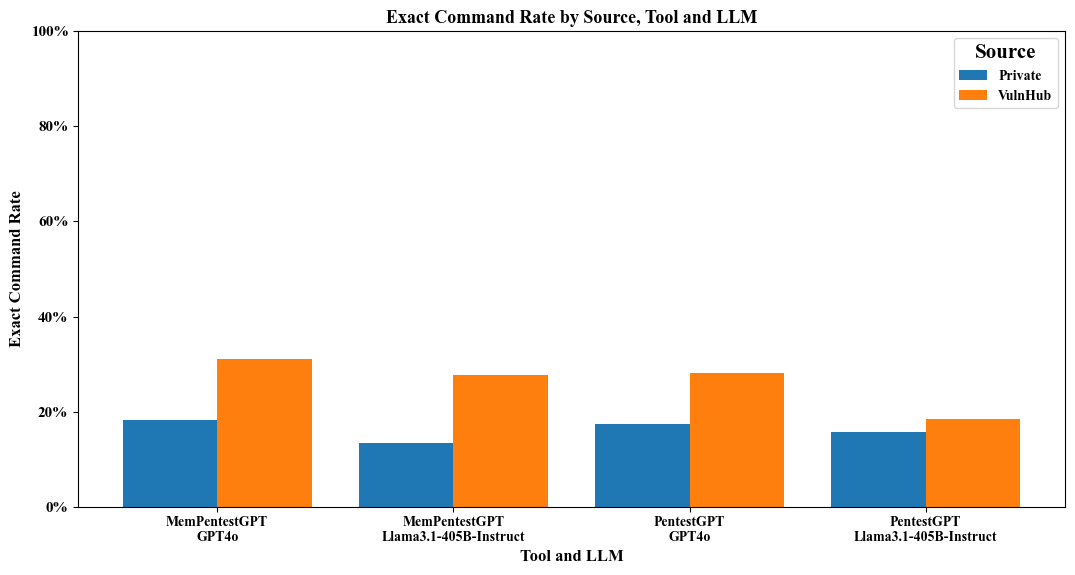
\includegraphics[width=0.5\textwidth]{exact_command_rate_by_machine_llm}
  \caption{Exact Command Rate by Machine and LLM}
  \label{fig:exact_command_rate_by_machine_llm}
\end{figure}

However, exact command matching should be interpreted carefully. The private machines also showed non-zero exact command rates, ranging roughly from 13\% to 18\% in Figure~\ref{fig:exact_command_rate_by_machine_llm}. Since these machines were privately created and were not expected to have public write-ups, exact matches in the private setting are more likely to come from common penetration-testing commands rather than memorised machine-specific solutions. For example, basic enumeration commands such as \texttt{sudo -l}, or standard privilege-escalation checks may naturally appear across many machines. \citet{happe_llms_2026} in their study also found that the LLMs often generate generate repeated basic enumeration commands. Therefore, exact command matching provides stronger evidence of memorisation when it occurs on public VulnHub machines and aligns with machine-specific write-ups, but it is weaker evidence when the matched command is a generic command commonly used in penetration testing. For example in easy3, both GPT4o and Llama-3.1 were failed to generate exact wordlist for path enumeration, unlike in Cengbox2 that GPT4o was able to suggest exact wordlist. 

Moreover, detail result show that the private machines exhibited little to no improvement in exact command rate when using MemPentestGPT. Among the private machines, only \textit{Easy1} showed an increase, from 0.0\% with PentestGPT to 6.2\% with MemPentestGPT. In contrast, \textit{Easy3} and \textit{Medium1} produced identical exact command rates across both tools, at 18.8\% and 25.0\%, respectively. Notably, \textit{Medium2} showed a decrease when using MemPentestGPT, with the exact command rate declining from 23.1\% to 15.4\%. This suggests that memory-triggering prompts did not substantially improve exact command reproduction on private machines. By contrast, the VulnHub machines generally showed higher exact command rates under MemPentestGPT. \textit{Cengbox2}, \textit{Library2}, and \textit{Symfonos2} all improved when using MemPentestGPT, while \textit{Sar} remained unchanged at 28.6\%, as shown in Table~\ref{tab:exact_command_rate_machine}.

\begin{table}[htbp]
  \centering
  \caption{Machine Exact Command Rates}
  \label{tab:exact_command_rate_machine}
  \begin{tabular}{llcc}
    \hline
    \textbf{Source} & \textbf{Machine Name} & \textbf{PentestGPT} & \textbf{MemPentestGPT} \\
    \hline

    \multirow{4}{*}{Private} & \textit{Easy1} & 0.0\% & \textbf{6.2\%} \\
    & \textit{Easy3} & 18.8\% & 18.8\% \\
    & \textit{Medium1} & 25.0\% & 25.0\% \\
    & \textit{Medium2} & \textbf{23.1\%} & 15.4\% \\
    \hline

    \multirow{4}{*}{VulnHub} & \textit{Cengbox: 2} & 31.2\% & \textbf{43.8\%} \\
    & \textit{The Library: 2} & 12.5\% & \textbf{18.8\%} \\
    & \textit{Sar} & 28.6\% & 28.6\% \\
    & \textit{Symfonos: 2} & 22.2\% & \textbf{27.8\%} \\
    \hline
  \end{tabular}
\end{table}

The outcome composition in Figure~\ref{fig:outcome_composition} reinforces this interpretation. Across all configurations, successful tasks were divided into two categories: successes with exact command matches and successes without exact matches. On VulnHub, the green segments, representing "success with exact match", were generally larger than on private machines. For example, VulnHub MemPentestGPT GPT-4o had the largest success-with-exact-match proportion, while private-machine configurations showed smaller exact-match proportions. Nevertheless, Figure~\ref{fig:outcome_composition} also shows that a substantial share of successful tasks did not involve exact command matching. This means that memorisation was detectable, but it did not explain all successful outcomes. The tools also appeared to use general penetration-testing patterns, partial reasoning, or non-identical commands that still advanced the attack.

\begin{figure}[htbp]
  \centering
  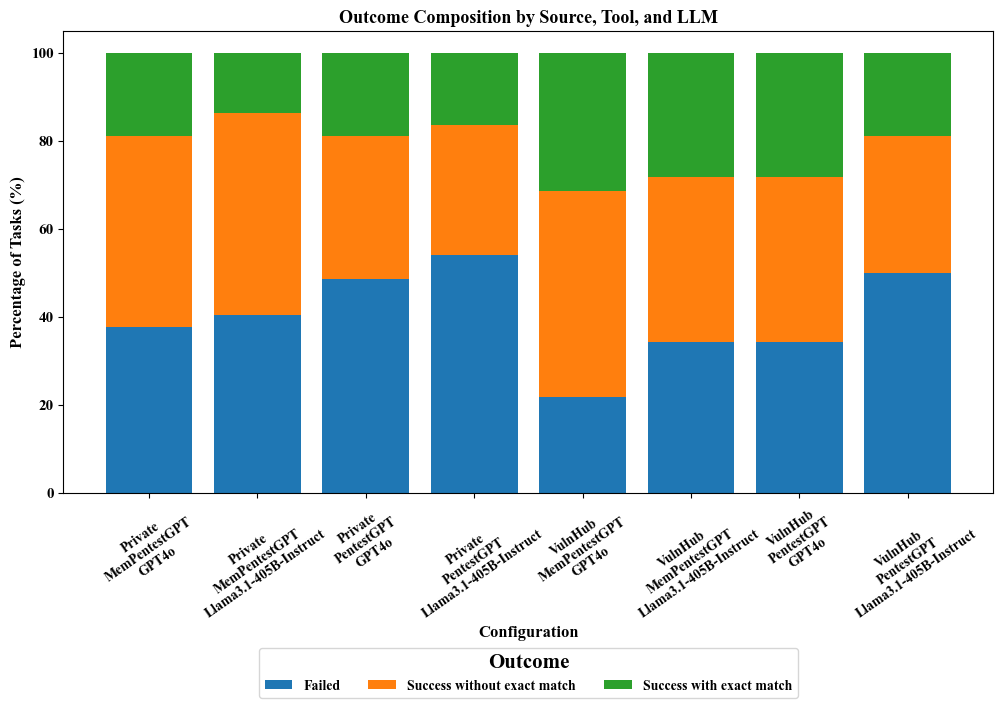
\includegraphics[width=0.5\textwidth]{outcome_composition_by_source_tool_llm}
  \caption{Outcome Composition by Source, Tool, and Model}
  \label{fig:outcome_composition}
\end{figure}

Overall, LLM-based penetration testing tools were moderately effective, particularly on public VulnHub machines. GPT-4o generally outperformed Llama-3.1-405B-Instruct, this is also in line with \citet{happe_llms_2026} where OpenAI models perform better in command generation than Meta-Llama model that sometimes often hallucinate and gives unknown self generated command. Study from \citet{nakano_guided_2025} also mentioned that GPT-4 is performing better than other models in solving HTB machines. Furhtermore, MemPentestGPT generally outperformed the baseline PentestGPT. The higher success rates, attempt success rates, and exact command rates on VulnHub suggest that public machines benefited from prior exposure to publicly available exploitation patterns. Ground-truth matching therefore reveals evidence of potential memorisation, especially for public machines with existing write-ups. However, memorisation was not the sole explanation for success, many successful tasks did not exactly match ground truth commands, and some exact matches on private machines were likely caused by generic suggestion commands, high-frequency penetration-testing commands. Thus, memorisation appears to be a measurable contributor to performance, but not the only mechanism driving tool effectiveness.


\subsection{RQ2. Mutation-Based Analysis}
In this section the study use MemPentestGPT because it was showing better result on previous section. Moreover, mutation-based test only tested on the successful task where both GPT-4o and Llama3.1-405B-Instruct had already succeeded under the original MemPentestGPT setting due to resource limitation. This section tests the adaptability of the tool when task information is constrained through masking or omission. Therefore, the results should be interpreted as an analysis of adaptability after baseline success, rather than as a general benchmark of penetration-testing capability. The details of the number of tasks tested is presented on Table~\ref{tab:total_tasks_by_machine}

\begin{table}[htbp]
  \centering
  \caption{Total Tasks by Source and Machine}
  \label{tab:total_tasks_by_machine}
  \begin{tabular}{llr}
    \hline
    \textbf{Source} & \textbf{Machine Name} & \textbf{Total Task} \\
    \hline
    \multirow{4}{*}{VulnHub}
    & \textit{The Library: 2} & 5 \\
    & \textit{Sar} & 7 \\
    & \textit{Symfonos: 2} & 6 \\
    & \textit{Cengbox: 2} & 10 \\
    \hline
    \multirow{4}{*}{Private}
    & \textit{Easy1} & 3 \\
    & \textit{Easy3} & 4 \\
    & \textit{Medium1} & 7 \\
    & \textit{Medium2} & 6 \\
    \hline
  \end{tabular}
\end{table}


\begin{figure}[htbp]
  \centering
  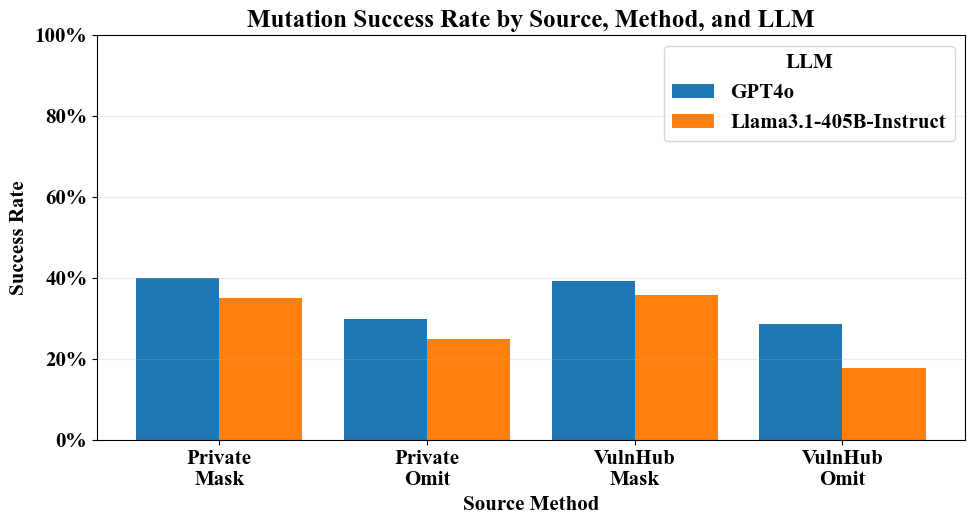
\includegraphics[width=0.5\textwidth]{mutation_success_rate_by_source_method_llm}
  \caption{Mutation based success rate}
  \label{fig:mutation_sr}
\end{figure}

As shown in Figure~\ref{fig:mutation_sr}, mutation reduced the success rate for both models across private and VulnHub machines. In both sources, the Mask setting produced higher success rates than the Omit setting. This suggests that both models were more capable of continuing the task when partial information was still available, while full omission of key contextual details made adaptation more difficult. GPT-4o consistently achieved higher success rates than Llama3.1-405B-Instruct, indicating stronger robustness under mutated task conditions. However, Llama3.1-405B-Instruct also have higher performance in private machines with omitting key details rather than in VulnHub. 

\begin{table}[htbp]
  \centering
  \caption{Mutation-Based Attempt Success Rates by Source and Model}
  \label{tab:mutation_success_rate}
  \begin{tabular}{llcc}
    \hline
    \textbf{Source} & \textbf{Method} & \textbf{GPT-4o} & \textbf{Llama-3.1} \\
    \hline
    \multirow{2}{*}{Private}
    & Mask & 11.3\% (8/71) & 9.3\% (7/75) \\
    & Omit & 7.7\% (6/78) & 6.3\% (5/79) \\
    \hline
    \multirow{2}{*}{VulnHub}
    & Mask & 11.5\% (11/96) & 9.3\% (10/107) \\
    & Omit & 7.5\% (8/106) & 4.2\% (5/119) \\
    \hline
  \end{tabular}
\end{table}

The attempt success rate result in Table~\ref{tab:mutation_success_rate} further shows that mutation affected efficiency. Attempt success rates were lower than task-level success rates for both models, particularly under Omit. This means that even when the tool eventually succeeded, it often required multiple attempts. Therefore, the observed successes should not be interpreted as consistently reliable adaptation, but rather as partial adaptation under constrained conditions.

\begin{table}[htbp]
  \centering
  \caption{Exact Command Rates under Mutation by Source and Model}
  \label{tab:mutation_exact_command_rate}
  \begin{tabular}{llcc}
    \hline
    \textbf{Source} & \textbf{Method} & \textbf{GPT-4o} & \textbf{Llama-3.1} \\
    \hline
    \multirow{2}{*}{Private}
    & Mask & 5.0\% (1/20) & 0.0\% (0/20) \\
    & Omit & 5.0\% (1/20) & 0.0\% (0/20) \\
    \hline
    \multirow{2}{*}{VulnHub}
    & Mask & 10.7\% (3/28) & 17.9\% (5/28) \\
    & Omit & 7.1\% (2/28) & 3.6\% (1/28) \\
    \hline
  \end{tabular}
\end{table}

The exact-command analysis in Table~\ref{tab:mutation_exact_command_rate} shows that exact command reproduction under mutation was limited overall. In the private-machine setting, exact command matches were almost absent: GPT-4o produced only one exact command match under both Mask and Omit conditions, while Llama-3.1-405B-Instruct produced no exact command matches. VulnHub produced higher exact-command rates than private machines, particularly under the Mask condition, where Llama-3.1-405B-Instruct reached the highest rate at 17.9\% (5/28), followed by GPT-4o at 10.7\% (3/28). Since VulnHub machines are public and commonly accompanied by online write-ups, exact command reproduction in this setting is more consistent with potential memorisation. In the other hand, the Omit condition reduced the exact-command rate for both models on VulnHub, suggesting that removing key information weakened the models ability to reproduce commands exactly. The private machines were newly constructed and often relied on standard commands.

However, these results should be interpreted cautiously. In the private machines, the few exact command matches were largely associated with basic penetration-testing commands, such as \texttt{sudo -l}, rather than machine-specific exploitation commands. Therefore, exact command matches in the private-machine setting do not necessarily provide strong evidence of memorisation. Instead, they may reflect the models use of common penetration-testing heuristics or standard privilege-escalation checks. By contrast, the higher exact-command rates on VulnHub, especially under the Mask condition, are more suggestive of potential memorisation because public machines are more likely to have existing write-ups and repeated solution patterns available online. For example, in the \texttt{Sar} machine, even after key details were masked, Llama-3.1-405B-Instruct generated a reverse-shell payload that closely resemble payloads reported in public write-ups, as shown below:

\begin{lstlisting}
?plot=;python3 -c 'import socket,subprocess,os;s=socket.socket(socket.AF_INET,socket.SOCK_STREAM);s.connect(("<ATTACKER-IP>",<LISTENER-PORT>));os.dup2(s.fileno(),0); os.dup2(s.fileno(),1); os.dup2(s.fileno(),2);p=subprocess.call(["/bin/bash","-i"]);'
\end{lstlisting}

\noindent This similarity provides stronger evidence of potential memorisation in the VulnHub setting \cite{reddy2024sar,iihack2020sar}.

In Figure~\ref{fig:mutation_outcome_composition} the experiment shown task cross configurations, which most tasks fell into the Failed category, indicating that both models struggled when information was constrained. The proportion of Success without exact match was generally larger than Success with exact match, suggesting that most successful mutation cases were not simply reproduced commands. However, Success with exact match still appeared, especially in VulnHub configurations. This indicates that memorisation may have helped in some public-machine tasks, but it was not the dominant source of success across all mutated tasks.

\begin{figure}[htbp]
  \centering
  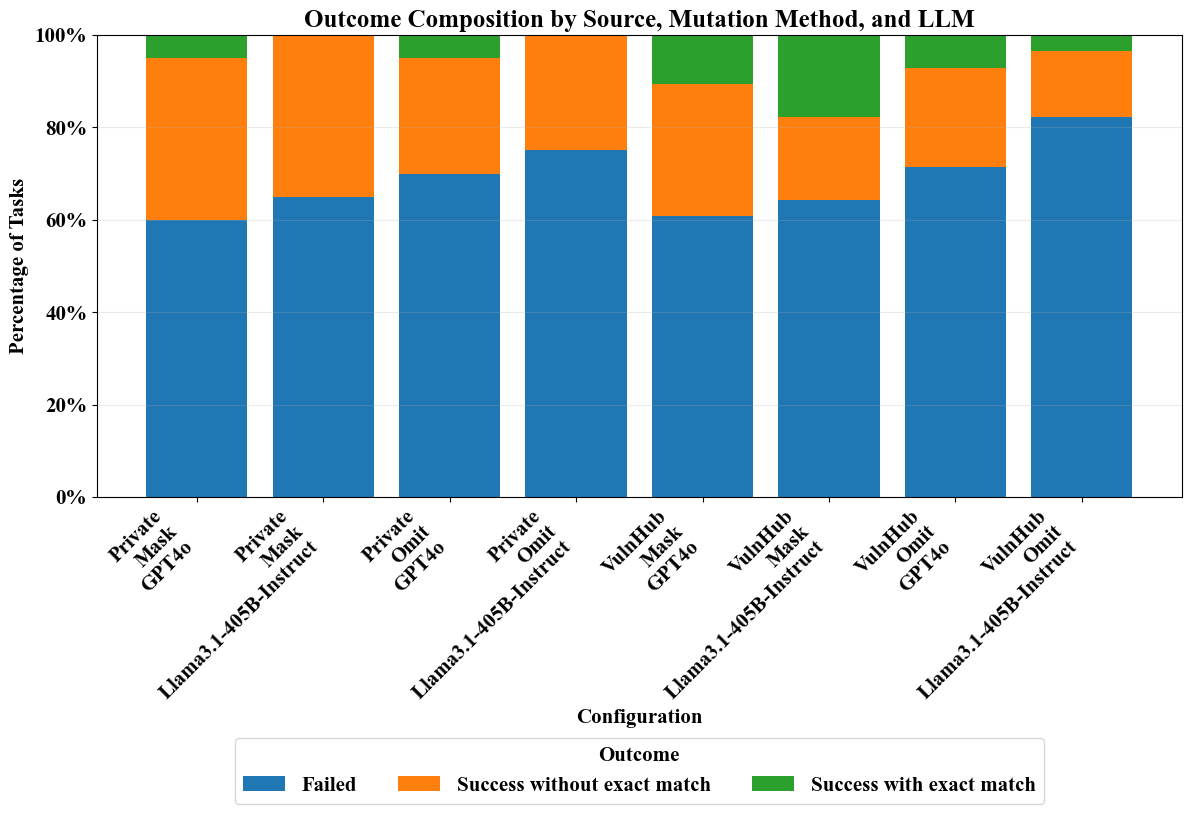
\includegraphics[width=0.5\textwidth]{mutation_outcome_composition_by_source_tool_llm.png}
  \caption{Mutation Outcome Composition}
  \label{fig:mutation_outcome_composition}
\end{figure}

The mutation-based results suggest that memorisation plays a limited and conditional role in MemPentestGPT. It can act as a strength when the mutated task still resembles a known public exploitation path, especially in VulnHub machines where public write-ups may exist. Therefore, MemPentestGPT shows partial adaptability under constrained information, but this adaptability is uneven. GPT-4o adapted better than Llama3.1-405B-Instruct, and Mask was less disruptive than Omit. Memorisation appears to be a strength mainly in public-machine scenarios where prior write-ups may guide the model toward known commands. However, when exact matches involve generic commands in private machines, it should not be treated as strong memorisation evidence. In this study, memorisation is therefore best interpreted as a conditional strength in familiar public environments, but a weakness when the task requires deeper adaptation beyond common commands or recalled exploitation patterns.

\section{Conclusion}


\section{Limitation}

This study encountered several limitations that could affect the interpretation of the results.
\begin{itemize}
  \item Each experimental condition was executed only once, without repeated trials. As LLM outputs can vary across runs, the absence of repetition limits the ability to measure output stability and statistical variation. Therefore, the results should be interpreted as indicative observations rather than definitive performance estimates.

  \item The experiments were conducted using PentestGPT version 0.14.0. As LLM-based penetration testing tools are actively developed, later versions may produce different results due to changes in prompting structure, tool integration, parsing behaviour, or task management.

  \item The testing process still required human intervention in PentestGPT 0.14.0. Although the LLM-based tools generated commands and suggested next steps, human judgement was needed to execute commands, interpret outputs, decide whether a task had progressed, and determine when no further useful suggestions were available. As a result, the evaluation reflects an assisted penetration testing.

  \item Responses differed across LLMs and tools even when they were tested on the same vulnerable machine. Because different models sometimes suggested different routes, commands, or task sequences, the experiment had to be adjusted based on the response produced in each case. This makes exact one-to-one comparison more difficult, as the tested commands were not always identical across models and tools.
\end{itemize}
%%
%% The acknowledgments section is defined using the "acks" environment
%% (and NOT an unnumbered section). This ensures the proper
%% identification of the section in the article metadata, and the
%% consistent spelling of the heading.
\begin{acks}
  To Indonesia Endowment Fund for Education (LPDP) for funding this research.
\end{acks}

%%
%% The next two lines define the bibliography style to be used, and
%% the bibliography file.
\bibliographystyle{ACM-Reference-Format}
\bibliography{references}


%%
%% If your work has an appendix, this is the place to put it.
\appendix

\end{document}
\endinput
%%
%% End of file `sample-acmtog.tex'.
